\documentclass[12pt, titlepage]{article}

\usepackage{fullpage}
\usepackage[round]{natbib}
\usepackage{multirow}
\usepackage{booktabs}
\usepackage{tabularx}
\usepackage{graphicx}
\usepackage{float}
\usepackage{hyperref}
\hypersetup{
    colorlinks,
    citecolor=blue,
    filecolor=black,
    linkcolor=red,
    urlcolor=blue
}

%% Comments

\usepackage{color}

\newif\ifcomments\commentstrue %displays comments
%\newif\ifcomments\commentsfalse %so that comments do not display

\ifcomments
\newcommand{\authornote}[3]{\textcolor{#1}{[#3 ---#2]}}
\newcommand{\todo}[1]{\textcolor{red}{[TODO: #1]}}
\else
\newcommand{\authornote}[3]{}
\newcommand{\todo}[1]{}
\fi

\newcommand{\wss}[1]{\authornote{blue}{SS}{#1}} 
\newcommand{\plt}[1]{\authornote{magenta}{TPLT}{#1}} %For explanation of the template
\newcommand{\an}[1]{\authornote{cyan}{Author}{#1}}

%% Common Parts

\newcommand{\progname}{Software Engineering} % PUT YOUR PROGRAM NAME HERE
\newcommand{\authname}{Team 15, ASLingo
\\ Andrew Kil
\\ Cassidy Baldin
\\ Edward Zhuang
\\ Jeremy Langner
\\ Stanley Chan} % AUTHOR NAMES                  

\usepackage{hyperref}
    \hypersetup{colorlinks=true, linkcolor=blue, citecolor=blue, filecolor=blue,
                urlcolor=blue, unicode=false}
    \urlstyle{same}
                                


\newcounter{acnum}
\newcommand{\actheacnum}{AC\theacnum}
\newcommand{\acref}[1]{AC\ref{#1}}

\newcounter{ucnum}
\newcommand{\uctheucnum}{UC\theucnum}
\newcommand{\uref}[1]{UC\ref{#1}}

\newcounter{mnum}
\newcommand{\mthemnum}{M\themnum}
\newcommand{\mref}[1]{M\ref{#1}}

\begin{document}

\title{Module Guide for \progname{}} 
\author{\authname}
\date{\today}

\maketitle

\pagenumbering{roman}

\section{Revision History}

\begin{tabularx}{\textwidth}{p{3cm}p{2cm}X}
\toprule {\bf Date} & {\bf Version} & {\bf Notes}\\
\midrule
Jan. 9, 2024 & 1.0 & Andrew and Edward; added module hierarchy\\
Jan. 10, 2024 & 1.1 & Stanley; added some module decompositions for hardware hiding and behaviour hiding modules\\
Jan. 10, 2024 & 1.2 & Andrew; rearranged Module Hierarchy and added decomposition descriptions for controller, hand sign recognition and verification modules\\
Jan. 11, 2024 & 1.3 & Jeremy and Cassidy added front end anticipated changes, modules and traceability mapping to these modules\\
Jan. 12, 2024 & 1.4 & Stanley; added some back end anticipated changes, more traceability mapping for functional requirements and modules\\
Jan 13, 2024 & 1.5 & Andrew; Added Uses Hierarchy Diagram\\
Jan 15, 2024 & 1.6 & Andrew; Cleaned up minor errors\\
Jan 17, 2024 & 1.7 & Jeremy; Replaced Login/Signup module with Authentication module. Added in Andrews updates UsesHierarchy image\\
Jan 17, 2024 & 1.8 & Cassidy; Added in Reference Material, Abbreviations, and Reflection Template\\
Jan 17, 2024 & 1.9 & Stanley; Answered reflection question 2\\
Jan 23, 2024 & 2.0 & Cassidy; Addressed git issue \#69 regarding AC1 module \\
Jan 23, 2024 & 2.1 & Cassidy; Addressed git issue \#49 regarding NFRT2 - PT3 and PR3 \\
\bottomrule
\end{tabularx}

\newpage

\section{Reference Material}

This section records information for easy reference. \\

%\noindent \href{https://github.com/stanreee/sign-language-learning/blob/main/docs/DevelopmentPlan/DevelopmentPlan.pdf}{Development Plan \citep*{DP}}\\

\noindent The \href{https://github.com/stanreee/sign-language-learning/blob/main/docs/DevelopmentPlan/DevelopmentPlan.pdf}{Development Plan} outlines the roles of each team member and the areas that each member will focus on. This breakdown of team responsibilities allows the team to assign testing roles accordingly. This document also contains the tools that the team plans on using for testing.\\

%\noindent \href{https://github.com/stanreee/sign-language-learning/blob/main/docs/SRS/SRS.pdf}{Software Requirements Specification \citep*{SRS}}\\

\noindent The \href{https://github.com/stanreee/sign-language-learning/blob/main/docs/SRS/SRS.pdf}{Software Requirements Specification} lists the functional and non-functional requirements which will aid in testing by formulating a testing plan to meet each requirement. Non-functional requirements should be tested such that the fit criteria are met.\\

%\noindent \href{https://github.com/stanreee/sign-language-learning/blob/main/docs/HazardAnalysis/HazardAnalysis.pdf}{Hazard Analysis \citep*{HA}}\\

\noindent The \href{https://github.com/stanreee/sign-language-learning/blob/main/docs/HazardAnalysis/HazardAnalysis.pdf}{Hazard Analysis} identifies failure modes to determine the implementation strategies to mitigate them. These will be used as a part of the testing plan to ensure that the failures are covered.\\

%\noindent \href{https://github.com/stanreee/sign-language-learning/blob/main/docs/Design/SoftDetailedDes/MIS.pdf}{Module Interface Specification \citep*{MIS}}\\

\noindent The \href{https://github.com/stanreee/sign-language-learning/blob/main/docs/Design/SoftDetailedDes/MIS.pdf}{Module Interface Specification} further decomposes the software's modules into specific access routines. The team will build the testing plan such that each function and routine works as intended.

\subsection{Abbreviations and Acronyms}

\renewcommand{\arraystretch}{1.2}
\begin{tabular}{|p{3cm}|p{13cm}|} 
  \toprule		
  \textbf{symbol} & \textbf{description}\\
  \midrule 
  AC & Anticipated Change\\
  ASL & Shorthand for American Sign Language. It is a form of sign language primarily used in the US and in parts of Canada. \\
  ASLingo & The commercial name for the project. \\
  CV & Refers to Computer Vision, the field of technology that invloves processing visual input ot achieve various means. \\
  HSR & Shorthand for "Health and Safety Requirements", a subsection of Non-Functional Requirements. \\
  FR & Shorthand for Functional Requirements. \\
  LR & Shorthand for "Legal Requirements", a subsection of Non-Functional Requirements. \\
  LFR & Shorthand for "Look and Feel Requirements", a subsection of Non-Functional Requirements. \\
  MSR & Shorthand for "Maintainability and Support Requirements", a subsection of Non-Functional Requirements. \\
  OER & Shorthand for "Operational and Environmental Requirements", a subsection of Non-Functional Requirements. \\
  OpenCV & Refers to the Open Computer Vision Library library available for free to developers in order to develop Computer Vision applications. \\
  M & Module \\
  MG & Module Guide \\
  PR & Shorthand for "Performance Requirements", a subsection of Non-Functional Requirements. \\
  SR & Shorthand for "Security Requirements", a subsection of Non-Functional Requirements. \\
  SRS & Software Requirements Specification\\
  UC & Unlikely Change \\
  UHR & Shorthand for "Usuability and Humanity Requirements", a subsection of Non-Functional Requirements. \\
  \bottomrule
\end{tabular}\\

\newpage

\tableofcontents

\listoftables

\listoffigures

\newpage

\pagenumbering{arabic}

\section{Introduction}

Decomposing a system into modules is a commonly accepted approach to developing
software.  A module is a work assignment for a programmer or programming
team~\citep{ParnasEtAl1984}.  We advocate a decomposition
based on the principle of information hiding~\citep{Parnas1972a}.  This
principle supports design for change, because the ``secrets'' that each module
hides represent likely future changes.  Design for change is valuable in SC,
where modifications are frequent, especially during initial development as the
solution space is explored.  

Our design follows the rules layed out by \citet{ParnasEtAl1984}, as follows:
\begin{itemize}
\item System details that are likely to change independently should be the
  secrets of separate modules.
\item Each data structure is implemented in only one module.
\item Any other program that requires information stored in a module's data
  structures must obtain it by calling access programs belonging to that module.
\end{itemize}

After completing the first stage of the design, the Software Requirements
Specification (SRS), the Module Guide (MG) is developed~\citep{ParnasEtAl1984}. The MG
specifies the modular structure of the system and is intended to allow both
designers and maintainers to easily identify the parts of the software.  The
potential readers of this document are as follows:

\begin{itemize}
\item New project members: This document can be a guide for a new project member
  to easily understand the overall structure and quickly find the
  relevant modules they are searching for.
\item Maintainers: The hierarchical structure of the module guide improves the
  maintainers' understanding when they need to make changes to the system. It is
  important for a maintainer to update the relevant sections of the document
  after changes have been made.
\item Designers: Once the module guide has been written, it can be used to
  check for consistency, feasibility, and flexibility. Designers can verify the
  system in various ways, such as consistency among modules, feasibility of the
  decomposition, and flexibility of the design.
\end{itemize}

The rest of the document is organized as follows. Section
\ref{SecChange} lists the anticipated and unlikely changes of the software
requirements. Section \ref{SecMH} summarizes the module decomposition that
was constructed according to the likely changes. Section \ref{SecConnection}
specifies the connections between the software requirements and the
modules. Section \ref{SecMD} gives a detailed description of the
modules. Section \ref{SecTM} includes two traceability matrices. One checks
the completeness of the design against the requirements provided in the SRS. The
other shows the relation between anticipated changes and the modules. Section
\ref{SecUse} describes the use relation between modules.

\section{Anticipated and Unlikely Changes} \label{SecChange}

This section lists possible changes to the system. According to the likeliness
of the change, the possible changes are classified into two
categories. Anticipated changes are listed in Section \ref{SecAchange}, and
unlikely changes are listed in Section \ref{SecUchange}.

\subsection{Anticipated Changes} \label{SecAchange}

Anticipated changes are the source of the information that is to be hidden
inside the modules. Ideally, changing one of the anticipated changes will only
require changing the one module that hides the associated decision. The approach
adapted here is called design for
change.

\begin{description}
\item[\refstepcounter{acnum} \actheacnum \label{acInfo}:] The ASL vocabulary included in the program may be updated in the future as the language evolves.
\item[\refstepcounter{acnum} \actheacnum \label{acAbout}:] The Landing Page Module may change if the developers want to change the formatting of the informational pages on the website (for example the home/resources page that use this module). 
\item[\refstepcounter{acnum} \actheacnum \label{acExercise}:] Exercise and Exercise Selection/History module may change if developers want to add in additional testing methods or material.
\item[\refstepcounter{acnum} \actheacnum \label{acAccount}:] Account management module may change if developers change what information is stored about the users progress. 
\item[\refstepcounter{acnum} \actheacnum \label{acMLModel}:] Structure of neural network in Machine Learning module may change to improve performance and accuracy.
\item[\refstepcounter{acnum} \actheacnum \label{acTestVerif}:] Test cases in the Testing and Verification module may change throughout development to improve code coverage as well as to cover any previously mentioned anticipated changes.
\end{description}

\subsection{Unlikely Changes} \label{SecUchange}

The module design should be as general as possible. However, a general system is
more complex. Sometimes this complexity is not necessary. Fixing some design
decisions at the system architecture stage can simplify the software design. If
these decision should later need to be changed, then many parts of the design
will potentially need to be modified. Hence, it is not intended that these
decisions will be changed.

\begin{description}
\item[\refstepcounter{ucnum} \uctheucnum \label{ucIO}:] Input/Output devices
  (Input: File and/or Keyboard, Output: File, Memory, and/or Screen).
\item[\refstepcounter{ucnum} \uctheucnum \label{ucLogin}:] The Authentication module is unlikely to change as we will be using user authentication methods and standard login procedures that are unlikely to change.
\end{description}

\section{Module Hierarchy} \label{SecMH}

This section provides an overview of the module design. Modules are summarized
in a hierarchy decomposed by secrets in Table \ref{TblMH}. The modules listed
below, which are leaves in the hierarchy tree, are the modules that will
actually be implemented.

\begin{description}
\item [\refstepcounter{mnum} \mthemnum \label{m1}:] Hand Sign Recognition Module
\item [\refstepcounter{mnum} \mthemnum \label{m2}:] Hand Sign Verification Module
% Need a middle-man to help frontend-backend communicate
% Ex: Front end changes the question, need to tell backend we're looking for a different sign now
\item [\refstepcounter{mnum} \mthemnum \label{m3}:] Controller Module
% Parsing raw data to processable data
\item [\refstepcounter{mnum} \mthemnum \label{m4}:] Data Collection Module
\item [\refstepcounter{mnum} \mthemnum \label{m5}:] Data Processing Module
\item [\refstepcounter{mnum} \mthemnum \label{m6}:] Machine Learning Module
\item [\refstepcounter{mnum} \mthemnum \label{m7}:] Testing and Verification Module
\item [\refstepcounter{mnum} \mthemnum \label{m8}:] Video Input Module
\item [\refstepcounter{mnum} \mthemnum \label{m9}:] Landing Page Module
\item [\refstepcounter{mnum} \mthemnum \label{m10}:] Exercise Module
\item [\refstepcounter{mnum} \mthemnum \label{m11}:] Exercise Selection/History Module
\item [\refstepcounter{mnum} \mthemnum \label{m12}:] Authentication Module
\item [\refstepcounter{mnum} \mthemnum \label{m13}:] Account Management Module
\end{description}

\begin{table}[h!]
\centering
\begin{tabular}{p{0.3\textwidth} p{0.6\textwidth}}
\toprule
\textbf{Level 1} & \textbf{Level 2}\\
\midrule

\multirow{1}{0.3\textwidth}{Hardware-Hiding Module} 
& Video Input Module \mref{m8}\\
\midrule

\multirow{4}{0.3\textwidth}{Behaviour-Hiding Module} 
& Hand Sign Recognition Module \mref{m1}\\
& Controller Module \mref{m3}\\
& Data Processing Module \mref{m5}\\
& Machine Learning Module \mref{m6}\\
& Landing Page Module \mref{m9}\\
& Exercise Module \mref{m10}\\
& Authentication Module \mref{m12}\\
\midrule

\multirow{3}{0.3\textwidth}{Software Decision Module} 
& Hand Sign Verification Module \mref{m2}\\
& Data Collection Module \mref{m4}\\
& Testing and Verification Module \mref{m7}\\
& Exercise Selection/History Module \mref{m11}\\
& Account Management Module \mref{m13}\\
\bottomrule

\end{tabular}
\caption{Module Hierarchy}
\label{TblMH}
\end{table}

\section{Connection Between Requirements and Design} \label{SecConnection}

The design of the system is intended to satisfy the requirements developed in
the SRS. In this stage, the system is decomposed into modules. The connection
between requirements and modules is listed in Table~\ref{TblRT}.

\section{Module Decomposition} \label{SecMD}

Modules are decomposed according to the principle of ``information hiding''
proposed by \citet{ParnasEtAl1984}. The \emph{Secrets} field in a module
decomposition is a brief statement of the design decision hidden by the
module. The \emph{Services} field specifies \emph{what} the module will do
without documenting \emph{how} to do it. For each module, a suggestion for the
implementing software is given under the \emph{Implemented By} title. If the
entry is \emph{OS}, this means that the module is provided by the operating
system or by standard programming language libraries.  \emph{\progname{}} means the
module will be implemented by the \progname{} software.

Only the leaf modules in the hierarchy have to be implemented. If a dash
(\emph{--}) is shown, this means that the module is not a leaf and will not have
to be implemented.

\subsection{Hardware Hiding Modules}

% \begin{description}
% \item[Secrets:]The data structure and algorithm used to implement the virtual
%   hardware.
% \item[Services:]Serves as a virtual hardware used by the rest of the
%   system. This module provides the interface between the hardware and the
%   software. So, the system can use it to display outputs or to accept inputs.
% \item[Implemented By:] OS
% \end{description}

\subsubsection{Video Input Module (\mref{m8})}
\begin{description}
\item[Secrets:] Image processing algorithms, software interaction with webcam hardware.
\item[Services:] Outputs real-time video data through user's webcam.
\item[Implemented By:] OpenCV and OS.
\end{description}

\subsection{Behaviour-Hiding Modules}

% \begin{description}
% \item[Secrets:]The contents of the required behaviours.
% \item[Services:]Includes programs that provide externally visible behaviour of
%   the system as specified in the software requirements specification (SRS)
%   documents. This module serves as a communication layer between the
%   hardware-hiding module and the software decision module. The programs in this
%   module will need to change if there are changes in the SRS.
% \item[Implemented By:] --
% \end{description}
\subsubsection{Hand Sign Recognition Module (\mref{m1})}
\begin{description}
\item[Secrets:] Recognises hand signs are being made.
\item[Services:] Relays the information that a hand sign is made.
\item[Implemented By:] Python and Pytorch.
\end{description}

\subsubsection{Controller Module (\mref{m3})}
\begin{description}
\item[Secrets:] Able to relay necessary information from back-end component to the correct corresponding front-end component and vice versa.
\item[Services:] Handles communication between front-end components and back-end components.
\item[Implemented By:] Python and JavaScript.
\end{description}

\subsubsection{Data Processing Module (\mref{m5})}
\begin{description}
\item[Secrets:] Algorithm used to process collected data.
\item[Services:] Formats datasets into usable training data for Machine Learning Module.
\item[Implemented By:] Python.
\end{description}

\subsubsection{Machine Learning Module (\mref{m6})}
\begin{description}
\item[Secrets:] Training data sets and structure of neural network.
\item[Services:] Takes in hand coordinate data and interprets and processes the data to return the appropriate letter.
\item[Implemented By:] Python and Pytorch.
\end{description}

\subsubsection{Landing Page Module (\mref{m9})}
\begin{description}
\item[Secrets:] Relevant information to shown to user about the program/website.
\item[Services:] Display necessary application information about ASLingo to the user on website.
\item[Implemented By:] Javascript.
\end{description}

\subsubsection{Exercise Module (\mref{m10})}
\begin{description}
\item[Secrets:] Question selection process and question bank used to quiz user.
\item[Services:] Creates an exercise module with questions based on current users level of progress.
\item[Implemented By:] Javascript.
\end{description}

\subsubsection{Authentication Module (\mref{m12})}
\begin{description}
\item[Secrets:] How user information is stored and accessed.
\item[Services:] Takes in user input to allow them to sign into their account.
\item[Implemented By:] Javascript.
\end{description}

\subsection{Software Decision Modules}

% \begin{description}
% \item[Secrets:] The design decision based on mathematical theorems, physical
%   facts, or programming considerations. The secrets of this module are
%   \emph{not} described in the SRS.
% \item[Services:] Includes data structure and algorithms used in the system that
%   do not provide direct interaction with the user. 
%   % Changes in these modules are more likely to be motivated by a desire to
%   % improve performance than by externally imposed changes.
% \item[Implemented By:] --
% \end{description}

\subsubsection{Hand Sign Verification Module (\mref{m2})}
\begin{description}
\item[Secrets:] The handshake used to determine whether the sign interpreted by the Machine Learning Module matches with the sign requested by front-end components
\item[Services:] Returns a pass/fail to front-end based on result of match attempt
\item[Implemented By:] Python
\end{description}

\subsubsection{Data Collection Module (\mref{m4})}

\begin{description}
\item[Secrets:] The un-processed training data collected.
\item[Services:] Stores collected data to be retrieved at a later time.
\item[Implemented By:] Python
\end{description}

\subsubsection{Testing and Verification Module (\mref{m7})}
\begin{description}
\item[Secrets:] Unit test cases used to test the software system.
\item[Services:] Verifies the software works as intended by testing the system on various test cases which ensures robustness, accuracy, and reliability.
\item[Implemented By:] Python and Pytest.
\end{description}

\subsubsection{Exercise Selection/History Module (\mref{m11})}
\begin{description}
\item[Secrets:] How historical data is stored for each user.
\item[Services:] Display users completed exercise progress and display current exercise options.
\item[Implemented By:] Javascript.
\end{description}

\subsubsection{Account Management Module (\mref{m13})}
\begin{description}
\item[Secrets:] How user information is stored and processed.
\item[Services:] Will keep a record of users account history after signing in to their account.
\item[Implemented By:] Javascript.
\end{description}

\section{Traceability Matrix} \label{SecTM}

This section shows two traceability matrices: between the modules and the
requirements and between the modules and the anticipated changes. 

In Table~\ref{TblACT}, the anticipated change \acref{acInfo} maps to multiple modules in our system. This change refers to the fact that ASL just like
many other languages is always evolving and changing over time. Because of this, if this system were to update the words or phrases that are used in
this application, it would affect the hand recognition models that were built on older data, as well as all the other modules that are affected by this model change. 

\begin{table}[H]
\centering
\begin{tabular}{p{0.2\textwidth} p{0.6\textwidth}}
\toprule
\textbf{Req.} & \textbf{Modules}\\
\midrule
FR1 & \mref{m8}\\
FR2 & \mref{m1} \mref{m6}\\
FR3 & \mref{m12}\\
FR4 & \mref{m12}\\
FR5 & \mref{m13}\\
FR6 & \mref{m10}\\
FR7 & \mref{m11}\\
FR8 & \mref{m13} \mref{m4}\\
FR10 & \mref{m2}\\
FR11 & \mref{m2}\\
FR12 & \mref{m11}\\
FR13 & \mref{m12}\\
LFR1 & \mref{m9}\\
LFR2 & \mref{m11}\\
LFR3 & \mref{m10}\\
UHR3 & \mref{m13}\\
UHR4 & \mref{m10}\\
SR1 & \mref{m12}\\
SR2 & \mref{m6}\\
SR3 & \mref{m13}\\
LR2 & \mref{m6}\\
PR2 & \mref{m6} \mref{m2}\\
OER2 & \mref{m8}\\
MSR3 & \mref{m7}\\
\bottomrule
\end{tabular}
\caption{Trace Between Requirements and Modules}
\label{TblRT}
\end{table}

\begin{table}[H]
\centering
\begin{tabular}{p{0.2\textwidth} p{0.6\textwidth}}
\toprule
\textbf{AC} & \textbf{Modules}\\
\midrule
\acref{acInfo} & \mref{m1}, \mref{m2}, \mref{m3}, \mref{m4}, \mref{m5}, \mref{m6}, \mref{m7},\\
\acref{acAbout} & \mref{m9}\\
\acref{acExercise} & \mref{m10}, \mref{m11}\\
\acref{acAccount} & \mref{m13}\\
\acref{acMLModel} & \mref{m6}\\
\acref{acTestVerif} & \mref{m7}\\
\bottomrule
\end{tabular}
\caption{Trace Between Anticipated Changes and Modules}
\label{TblACT}
\end{table}

\section{Use Hierarchy Between Modules} \label{SecUse}

In this section, the uses hierarchy between modules is
provided. \citet{Parnas1978} said of two programs A and B that A {\em uses} B if
correct execution of B may be necessary for A to complete the task described in
its specification. That is, A {\em uses} B if there exist situations in which
the correct functioning of A depends upon the availability of a correct
implementation of B.  Figure \ref{FigUH} illustrates the use relation between
the modules. It can be seen that the graph is a directed acyclic graph
(DAG). Each level of the hierarchy offers a testable and usable subset of the
system, and modules in the higher level of the hierarchy are essentially simpler
because they use modules from the lower levels.

\begin{figure}[H]
\centering
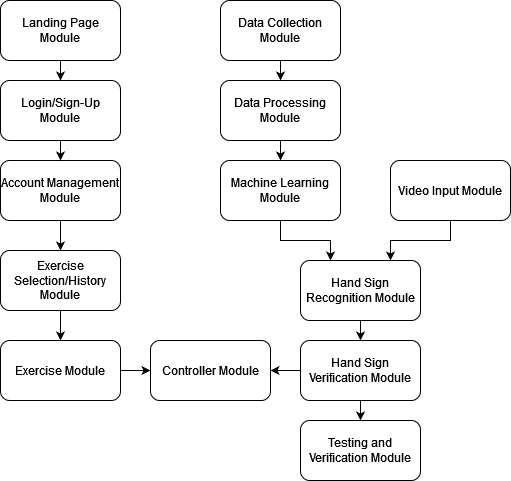
\includegraphics[width=0.7\textwidth]{UsesHierarchy.png}
\caption{Use hierarchy among modules}
\label{FigUH}
\end{figure}

\section{Timeline}
This timeline is under the assumption that this is all implemented for a single learning exercise which is what we projected in our expectations.

\begin{itemize}
    \item \textbf{Monday, Jan 22}
    \begin{itemize}
        \item Back-end  : Data Collection and Data Processing Modules Completion
        \item Front-end : Landing Page Module, Authentication Module Completion
    \end{itemize}
    \item \textbf{Friday, Jan 26}
    \begin{itemize}
        \item Back-end  : Machine Learning Module Completion
        \item Front-end : Account Management Module completion
    \end{itemize}
    \item \textbf{Monday, Jan 29}
    \begin{itemize}
        \item Back-end  : Video Input Module Integration
        \item Front-end : Exercise Selection/Menu Completion
    \end{itemize}
    \item \textbf{Friday, Feb 2}
    \begin{itemize}
        \item Back-end  : Hand Sign Recognition + Verification Module Completion
        \item Front-end : Exercise Module Completion
    \end{itemize}
    \item \textbf{Revision 0 Presentation : February 5th - February 16th}
    \item \textbf{Verification and Testing : Feb 19 - Feb 23}
\end{itemize}
\textbf{\textit{Further Scheduling done when dates draw closer to ensure realistic expectations}}

\section{Reflection}

The information in this section will be used to evaluate the team members on the
graduate attribute of Problem Analysis and Design.  Please answer the following questions:

\begin{enumerate}
  \item What are the limitations of your solution?  Put another way, given
  unlimited resources, what could you do to make the project better? (LO\_ProbSolutions)\\
  There are a few improvements we could implement given more time and resources. One of the main limitations of our design is that we
  do not have separate modules for dealing with static and dynamic hand signs. A perfect solution would recognize the expected type of
  hand sign and deal with the corresponding type individually. Static and dynamic hand signs are dealt with differently as for static signs,
  individual frames are what the machine learning model looks at, and for dynamic signs, the model should look at groupings of frames.\\
  Another limitation of our design is having one single controller module to connect the frontend with the backend. While this simplifies our
  work in design, given unlimited time, it would be ideal to have data sent through multiple controller modules, wherever a frontend/backend
  connection needs to be facilitated.
  \item Give a brief overview of other design solutions you considered.  What
  are the benefits and tradeoffs of those other designs compared with the chosen
  design?  From all the potential options, why did you select documented design?
  (LO\_Explores)\\
  One particular design solution we had in mind for the transfer of webcam frame data from the frontend to the backend was to
  only read the user's hand signs after a specified countdown timer, where the system would then send the current frame to the
  backend. This would avoid the need of sending each frame to the backend, improving performance. Although this would work with
  static hand signs (most letters of the alphabet), dynamic hand signs which involve the movement of hands to be tracked, would fail
  to be recognized. As such, we decided to continue with the original plan of sending each frame to the backend, and dealing with
  any potential performance issues during implementation.\\
  We also initially assumed that the middleman module between the frontend and the backend would only use the frontend and backend modules,
  and not vice versa where the frontend/backend modules would use the controller module. This was not the case, as we ran into
  scenarios where the hand sign verification module and the exercise module would require the use of certain functions in the controller
  module.
\end{enumerate}

\bibliographystyle {plainnat}
\bibliography{../../../refs/References}

\newpage{}

\end{document}
